\chapter{Ma collaboration au projet}\label{collab}
\putminitoc
Après avoir défini plus en détails les besoins de notre plateforme et son fonctionnement général, nous allons maintenant voir en détail de quelle manière j'ai contribué à ce projet. En parallèle de la maintenance de notre plateforme, j'ai développé deux nouvelles fonctionnalités. Ces deux fonctionnalités ayant un rapport direct avec la notion de << calibration >>, nous allons tout d'abord définir celles-ci avant de voir en détail mon développement et la maintenance que j'ai effectué.

\section{Les calibrations}
Une calibration est une constante stockée en flash, c'est-à-dire en mémoire non volatile. Ainsi le logiciel du contrôle moteur peut accéder à toutes ces calibrations en lecture uniquement.

Ces calibrations servent à configurer un véhicule avant sa mise en production, permettant la variabilité du logiciel à plusieurs niveaux : 
\begin{itemize}
	\item Configurer un calculateur pour tous les types de véhicule qu'il doit supporter. Certains ECU couvrent depuis l'entrée de game jusqu'au milieu de game d'un ou plusieurs constructeurs\footnote{Renault, Niassan et Dacia par exemple}. On peut configurer la présence ou l'absence de turbo, le nombre d'injecteurs, la taille des roues\ldots\newline
	 Autant de paramètre qui influent sur les lois de contrôle implantées dans l'ECU
	\item Ajuster le fonctionnement d'une loi de contrôle sur banc moteur ou sur véhicule pour tenir compte des normes de polution par exemple
	\item Tracer le calculateur en cas de retour fournisseur, ceci via des informations logistiques (Numéro de série, version du logiciel, \ldots)
\end{itemize}

Une fois le logiciel d'un calculateur mis en production, ces calibrations ne doivent pas évoluer, les modifier ne sert donc qu'à la mise au point et à la généricité du logiciel.
\vfill
\section{Le << patch calib >>}\label{patch}
Pour plusieurs scénarii de stimulation, il est nécessaire de modifier des valeurs de calibrations. Cette action demande d'ajouter une grammaire spécifique : \texttt{PATCH\_CAL(calibration, valeur)}. En interne, cela générera du code permettant de flasher la nouvelle valeur.
%
\subsection{Expression du besoin}\label{besoin-patch}
\subsubsection{Les cas d'utilisation}
		Comme nous pouvons le voir figure \ref{fig:patch-cal-usecase}, le patch de calibrations est répertorié en deux grandes parties : le parser avec la génération des instructions permettant de changer la valeur d'une calibration, et l'exécution du patch proprement dit.
		\begin{figure}[H]
			\centering
			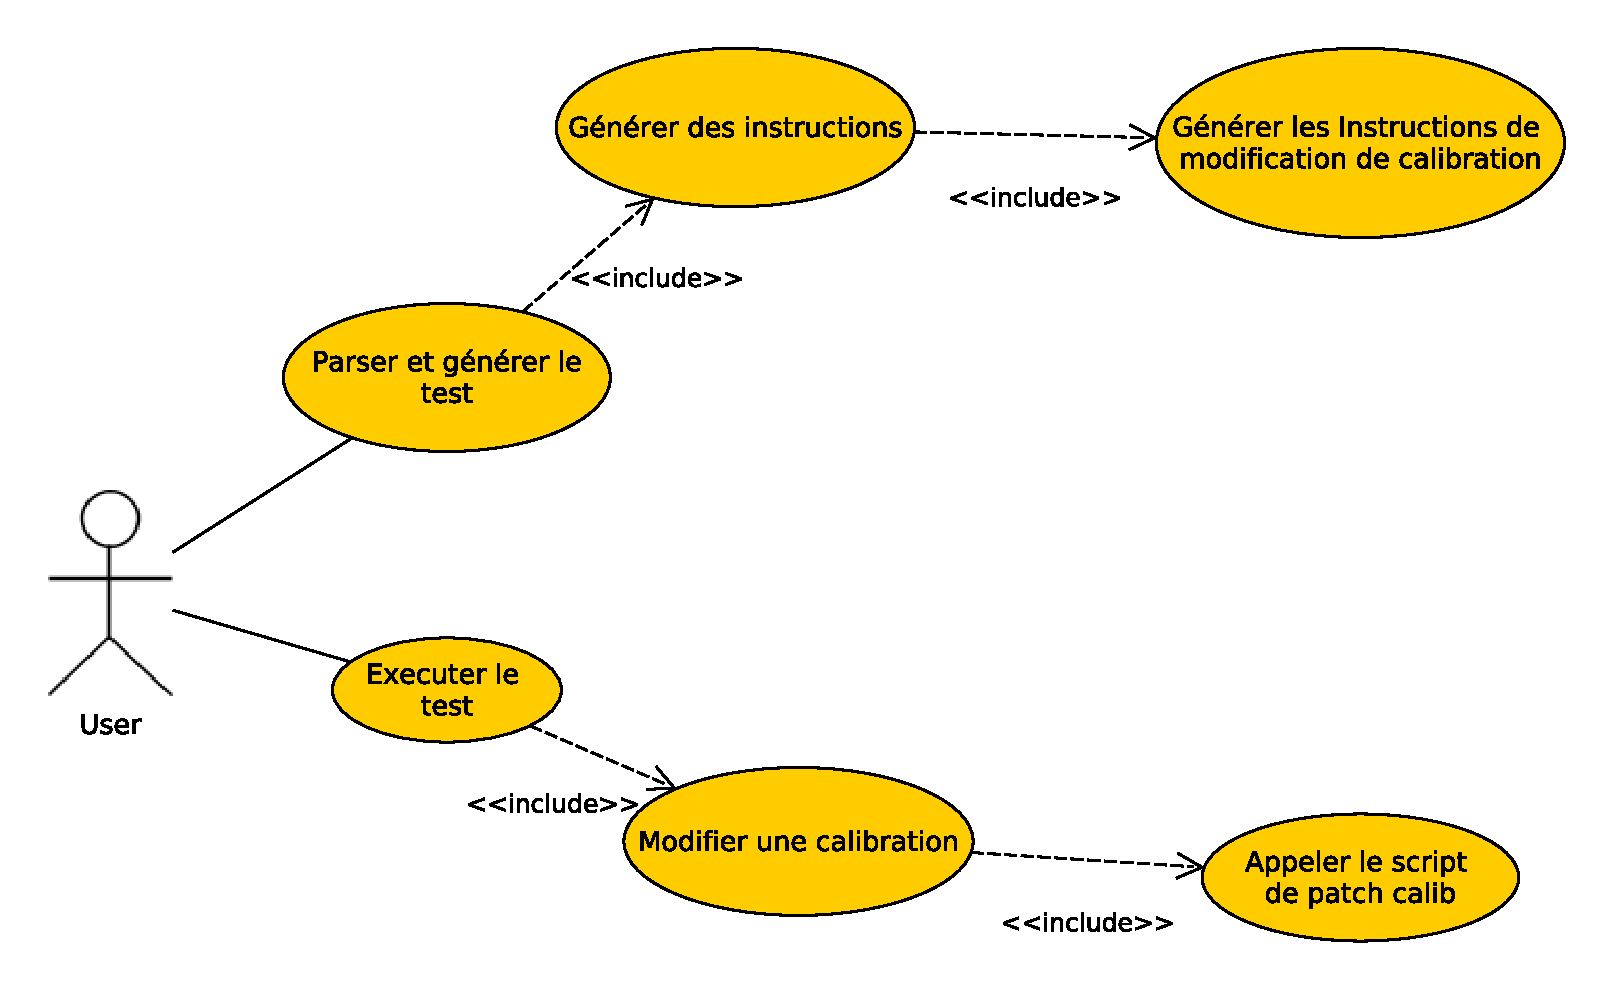
\includegraphics[width=12cm]{contents/images/patch-cal_usecase.eps}
			\caption{Diagramme de cas d'utilisations du patch de calibrations}
			\label{fig:patch-cal-usecase}
		\end{figure}

		\subsubsection{Limitations du \textit{patch calib}}\label{ecustop}
		Afin de concevoir au mieux la solution répondant aux besoins du client, j'ai tout d'abord dû me renseigner sur la manière dont je pouvais effectuer cette action sur l'ECU, et donc l'implémentation du serveur. Après discussions avec les personnes compétentes, une restriction impactant mon développement a été mise au clair.
		
		Afin de modifier une calibration, il est nécessaire de modifier la mémoire flash. Cette modification va nous obliger à éteindre l'ECU, la modification de la flash étant impossible ECU démarré. Il ne sera donc pas possible de modifier une calibration au milieu d'un scénario de stimulation, le scénario n'aurait aucun sens si nous éteignons et rallumons l'ECU pendant celui-ci.
		
		Cette restriction n'a cependant pas d'impact sur les tests qui seront rédigés, un scénario de stimulation a pour but de se rapprocher du fonctionnement nominal d'une voiture. Or il est inconcevable de modifier une calibration pendant que la voiture tourne. Du point de vue des tests, ce choix reste cohérent. 

\subsection{Fonctionnement à l'utilisation}\label{usePatch}
\vspace{-15px}
Comme vu section \ref{ecustop}, le << patch calib >> ne peut être utilisé que si l'ECU est arrêté. Afin de forcer ce fonctionnement, et d'éviter une mauvaise utilisation, il a été choisi d'utiliser la grammaire du langage. En effet, une mauvaise utilisation de la fonctionnalité nous renverra une \textit{syntax error}, forçant l'utilisateur à corriger cela. Cette grammaire effectuera implicitement l'arrêt et le redémarrage de l'ECU.

\begin{lstlisting}[language=gtl,numbers=left,caption=Scénario de stimulation contenant des patchs de calibration]
SCENARIO NomDuScenario
  PATCH SECTION
    patch_cal(cal1, value1);
    patch_cal(cal2, value2);
  END SECTION
  // Stimulation proprement dite
  // Rampe, wait, ...
END SCENARIO
\end{lstlisting}
L'utilisateur à la possibilité d'écrire plusieurs scénarii dans un même test, avec cette même syntaxe. Cette fonctionnalité permettra à un testeur de vérifier plusieurs stratégies en fonction de calibrations.
\vspace{-30px}
\subsection{Conception de la solution}
		\begin{wrapfigure}{r}{5.5cm}
			\vspace{-20px}
			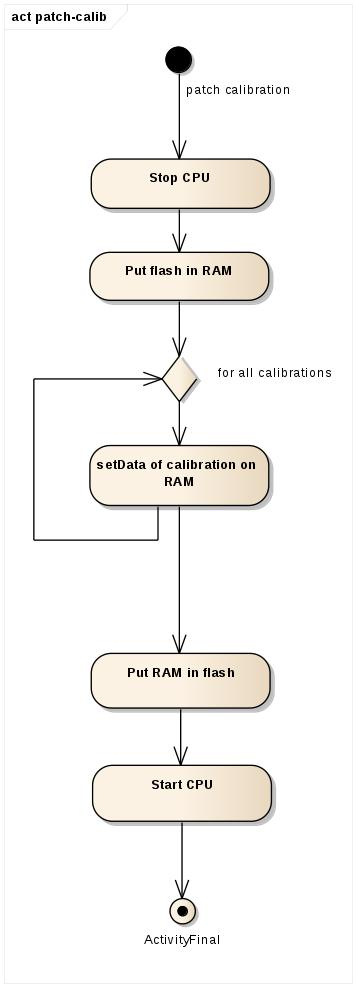
\includegraphics[height=14.2cm]{contents/images/script_activite.jpg}
			\caption{Diagramme d'activité du patch calib}
			\label{fig:scriptBatch} 
			\vspace{-3.5cm}
		\end{wrapfigure}
	Nous avons vu dans la section \ref{besoin-patch} que la fonctionnalité était répartie en deux grandes parties, le parser et l'exécution. Ces deux parties peuvent également s'apparenter à deux modules bien distincts de \textit{GreenT} : le client, pour le parser, et le serveur Debugger, pour l'exécution. Dans la suite de ce document, nous feront abstraction de l'utilisation de Thrift pour la communication réseau, celle-ci étant généré comme expliqué section \ref{thrift}.
	
	\subsubsection{Le serveur T32 : Exécution}
	Comme vu section \ref{T32server}, le serveur du debugger utilise l'outil Trace32. C'est cet outil qui nous permet d’interagir avec le calculateur embarqué. Cet outil fonctionne principalement en utilisant des scripts batch.\\
	Depuis l'interface de cet outil, il est possible de patcher une calibration.

	\begin{description}
		\item[Le script existant] Ce script a été pensé pour le mode graphique. L'utilisateur appelle le script, modifie les valeurs des calibrations voulues via l'interface , et clique sur «~patch intern flash~». À ce moment là, le patch en flash s'effectue.
		\item[Le nouveau script] Le nouveau script va effectuer les mêmes actions que le script existant, mais sans aucune attente d'actions utilisateurs. Pour cela, plutôt que d'attendre que l'utilisateur modifies les calibrations, nous aurons une liste calibration à modifier en paramètre.
	\end{description}

	Afin de modifier une calibration, présente en flash, un certain nombre d'actions sont nécessaires. Ces actions sont montrées dans le diagramme d'activité figure \ref{fig:scriptBatch}.
	
	Le service du serveur va ainsi appeler le nouveau script de patch, le code Java concerné sera donc minime. Le prototype de la méthode est la suivante : 
	\begin{lstlisting}[language=Java, numbers=none]
public void patchCalibs(Map<String, Long> calibs);
	\end{lstlisting}

	\subsubsection{Le client : Parser \& générateur}
	Afin de gérer le parsing et la génération de notre patch calib, j'ai dû créer une nouvelle règle de grammaire comme montré section \ref{usePatch}. 
	
	Avec cette nouvelle grammaire, j'ai forcé l'utilisateur à ne modifier des calibrations que si l'ECU est éteint, cette action n'étant possible que dans une \texttt{patch section}. Une fois la liste de calibrations à patcher parsée, il m'a suffit de générer l'instruction d'appel du Debugger.
	
	\begin{lstlisting}[language=Java]
Map<String, Long> calibrations = new HashMap<String, Long>();
calibrations.put("calib1", 0x0);
calibrations.put("calib2", 0x1);
dbg.patchCalibs(calibrations);
// Stimulation instructions
	\end{lstlisting}
	
	Pour répondre à un besoin de l'équipe cliente, j'ai ajouté une sauvegarde de la valeur des calibrations avant le premier scénario, et une restauration à la fin du dernier scenario. Ceci pour garantir une bonne cohérence, en effet, si l'utilisateur modifie une calibration, celle-ci doit revenir à la valeur initiale pour les tests suivants. Cette restauration se fait de façon implicite afin de limiter le travail des testeurs, qui pourrait être source d'erreur.
	
	Cette sauvegarde se fait simplement, en début de test, je lis la valeur de chacune des calibrations qui seront modifiées par la suite, à la fin du test, je patch chacune des valeurs de sauvegardes en appelant le service.
	
	\subsection{Les difficultés rencontrées}
	Afin de développer cette fonctionnalité, j'ai eu quelques problèmes à résoudre. Nous allons voir ici de quelle manière je m'y suis pris.
	\subsubsection{Le batch}
	Tout d'abord, j'ai du modifier un script batch, dans un langage que je ne connaissais pas, manipulant un outil que je ne connaissais pas. Afin de pouvoir effectuer mon nouveau script, j'ai donc lu la documentation de l'outil Trac32 expliquant le fonctionnement de leurs scripts, et la manière de les développer. J'ai également étudié le fonctionnement du script existant afin de l'adapter. J'ai eu la chance que celui-ci soit clair et assez bien construit. J'ai donc été rapidement opérationnel pour comprendre ce que faisait le script, et ce que j'allais devoir faire.
	
	\subsubsection{La robustesse}
Un problème plus important à cependant été soulevé assez rapidement. Nous avons choisis d'adapter un script Trace32 afin d'être le plus rapide possible, cependant celui-ci nous à soulevé un certain nombre de questions.

En effet, si nous effectuons un patch, que nous coupons l'allimentation de l'ECU, mettons l'allimentation de nouveau, et que nous essayons d'effectuer un nouveau patch, une erreur est levée, des bits d'erreurs mis à un, et l'ECU passe dans un état incohérent. 

Après investigation, nous avons pu cerner plusieurs sources éventuelles de ce problème : 
Il se pourrait qu'après la coupure de l'allimentation, les patchs suivants soient refusés en raison d'état de la RAM ou de la flash incohérent. 

Ce problème pourrait être localisé dans plusieurs endroits.
\begin{description}
\item[Le script existant] Ce script est peu utilisé par les équipes projet, ainsi, il n'est que peu testé. Il se pourrait que nous nous soyions basé sur un script possédant des bogues.
\item[Le driver flash propriétaire] Ce script utilise un driver flash propriétaire, dont nous ne connaissons pas exactement les actions. Il se pourrait que le problème vienne également de lui.
\end{description}

Ce problème semble donc compliqué à résoudre, une des solutions étant de développer notre propre driver flash afin d'avoir un contrôle de bout en bout. Cette solution étant particulièrement compliquée et couteuse, j'ai trouvé une autre solution beaucoup plus simple.\newline La coupure de l'allimentation de l'ECU provoque un état incohérent de la RAM, cependant, si nous redémarrons manuellement l'outil Trace32 entre deux patch, sans coupure brusque, le problème est résolu. Certainement car le démarrage de celui-ci nettoie certains secteurs. Cette solution n'est pas parfaite, mais a pu être effectuée rapidement et fonctionne correctement. Le jour ou de la robustesse sera particulièrement nécessaire, nous devrons développer notre propre driver.

\section{Les << tableaux calibrables >>}
Certaines variables côtés ECU sont des variables de types tableau, l’utilisateur peut actuellement y accéder via la syntaxe \texttt{var[indice]}.

Le but de mon développement était d’améliorer ce système. Actuellement, seul un indice numérique peut être renseigné à ce tableau, notre client souhaite pouvoir renseigner un indice sous forme d'entier ou d'une calibration.

\subsection{Expression du besoin}\label{besoinTab}
L'intérêt de renseigner une calibration comme indice de tableau est d’avoir les mêmes calibrations d’un projet, ou d'une \textit{release}, à l’autre, et de pouvoir réutiliser le \textit{Walkthrough} en ne changeant que les valeurs de ces calibrations.\\
Un autre avantage de cette fonctionnalité, est de pouvoir recopier scrupuleusement les spécifications, celles-ci étant renseignées via des calibrations.

Avec cette fonctionnalité, l'utilisateur pourra donc avoir des fichiers \textit{Walkthrough} génériques et réutilisables entre chaque version d'un même projet. Cela limitera également le risque d'erreurs dues à une mauvaise recopie de la spécification. En effet, avant cette fonctionnalité, l'utilisateur devait regarder la spécification, aller voir la valeur de la calibration, et la mettre en dur dans le test. Cela peut provoquer des erreurs, d'une part lors de mauvaise recopie de la valeur, mais également si la valeur change à la version suivante et que l'utilisateur oubli de modifier le \textit{Walkthrough}.

Ce besoin concerne uniquement les variables Debugger, et nullement le HiL. En effet, le debugger accède à des variables présentes dans le logiciel, dont des tableaux, il est nécessaire de pouvoir y accéder. Cependant, le HiL lui ne connait pas ce mécanisme, il n'utilise que des adresses afin d'accéder à ces élements de stimulation.

\subsubsection{Les cas d'utilisation}
\begin{figure}[H]
\centering
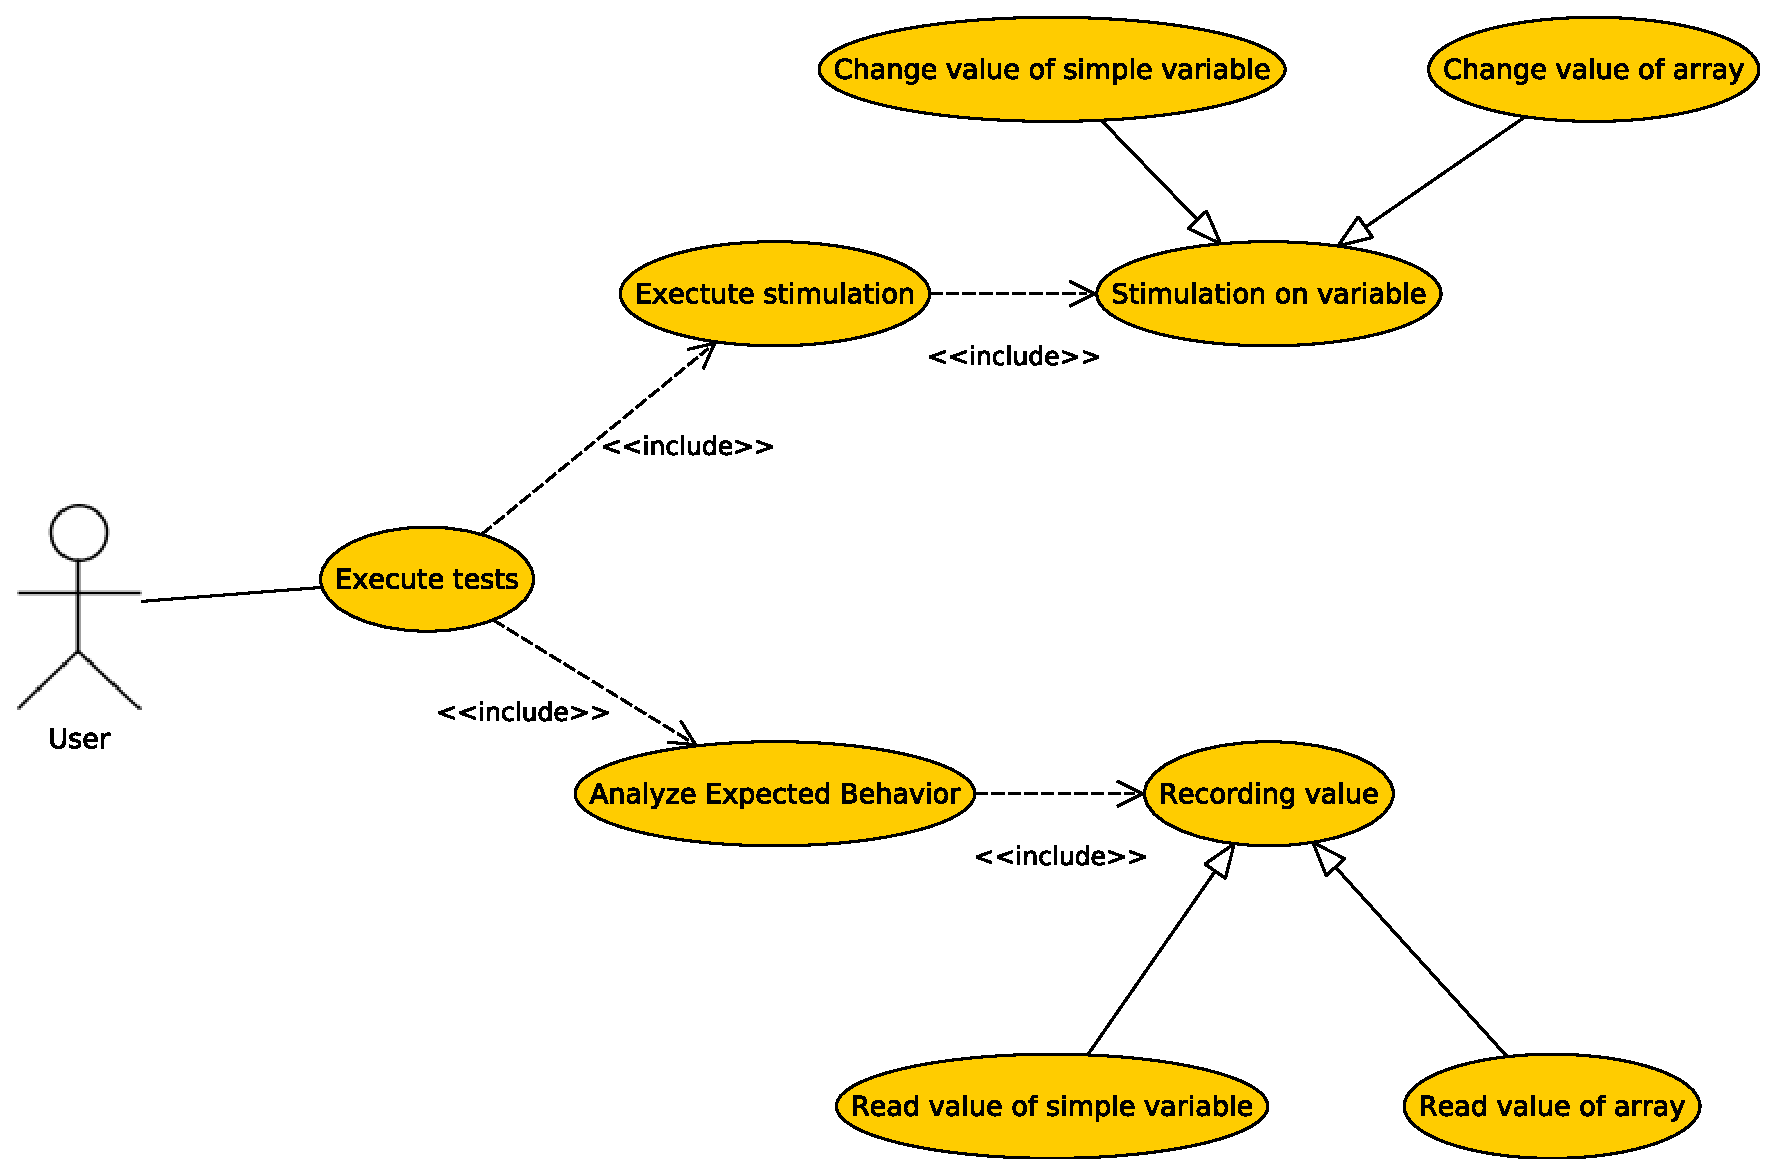
\includegraphics[width=18cm]{contents/images/usecasearray.eps}
\caption{Diagramme de cas d'utilisation des tableaux calibrables}
\end{figure}
\begin{remarque}
Cette fonctionnalité possède un cas d'erreurs qui devra être géré convenablement : 
\begin{itemize}
\item Si l'utilisateur renseigne un indice en dehors de la taille du tableau, une exception devra être levée
\item Si l'utilisateur renseigne autre chose qu'un entier ou une calibration en tant qu'indice, une erreur doit être levée au parsing\footnote{C'est à la grammaire du langage de ne pas autoriser d'autres indices}.
 \end{itemize}
 \end{remarque}
 
 Comme nous pouvons le voir dans ce diagramme de cas d'utilisation, le problème est découpé en deux sous-problèmes : 
 \begin{itemize}
 	\item L'exécution d'une stimulation, modifier une variable tableau sur le debugger, durant un scénario de stimulation. 
 	\item L'analyse de l'\textit{Expected Behavior}, c'est-à-dire un type de variable particulier au sein de notre expression logique.
 \end{itemize}
 

\subsection{Conception de la solution}
\subsubsection{L'exécution d'une stimulation}
Afin de pouvoir utiliser des tableaux à l'intérieur d'une stimulation j'ai ajouté de nouveaux Alias comme présenté figure \ref{fig:aliasClasses}. Pour éviter d'eventuels problèmes, je n'ai pas modifié l'existant, simplement ajouté la nouvelle fonctionnalité au sein de ce diagramme de classes, comme vous pouvez le voir avec les classes situées au centre, représentées en orange.

Un alias est un objet qui permet de faire l'abstraction entre le \textit{device} et l'action que l'on veut faire. Ainsi, ceux-ci sont répartis d'une part par \textit{device}, et d'autre part en fonction de leur mode d'accès, en lecture ou en écriture. Si un jour un nouveau \textit{device} est nécessaire, il faudra l'ajouter dans cet arbre d'héritage. Ces alias peuvent effectuer certaines actions en fonction du device concerné, tel que des modifications en physique, en hexadécimal ou en eléctrique, et des lectures de valeurs.

Durant ce stage, j'ai ajouté une abstraction permettant de séparer le fonctionnement des Alias << simple >> d'un côté, et ceux représentant un tableau. Un tableau pouvant être lui aussi accessible en lecture, ou en écriture. À noter que toutes les actions effectués sur ces alias vont vérifier que l'index demandé existe bel et bien, si ce n'est pas le cas une exception est renvoyée. 
% Diagramme de classes
\begin{figure}[H]
\hspace{-35px}
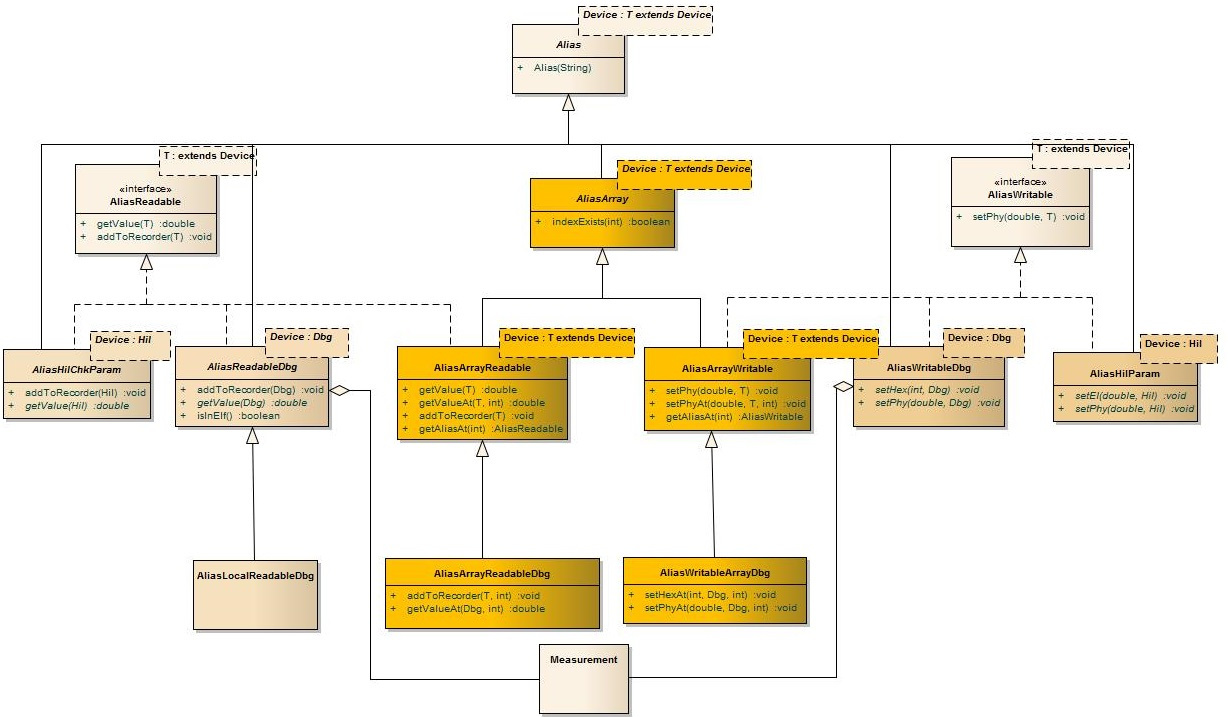
\includegraphics[width=20.5cm]{contents/images/alias.jpg}
\caption{Diagramme de classes -- Gestion des Alias}
\label{fig:aliasClasses}
\end{figure}

Ainsi, les tableaux s'utilisent assez facilement : si nous souhaitons accéder à un élément d'un tableau, il faut appeler les méthodes correspondantes : \texttt{setPhyAt}, \texttt{getValueAt}, \ldots Ces méthodes nécessitent un index, et c'est dans cette méthode que je vais effectuer un calcul d'adresse afin d'effectuer mes modifications sur la bonne variable.


% Diagramme de séquence
\subsubsection{L'analyse de l'\textit{Expected Behavior}}


\paragraph{Le stockage de la valeur du tableau} Afin d'enregistrer des valeurs durant un scénario, nous utilisons le Debugger, celui-ci génère une trace, que nous transformons ensuite en CSV. Les noms de chaque colonne sont impérativement le nom de la variable vu par le debugger, c'est-à-dire \texttt{variable} ou \texttt{tableau[0]}.

L'évaluation de notre \textit{Expected Behavior} se fera en local. Or, nous n'aurons pas la valeur de notre calibration, il sera donc impossible de faire le lien entre \texttt{tableau[0]} et \texttt{tableau[calib]}, même si \texttt{calib} vaut bien 0.

La solution la plus simple pour régler ce problème est d'enregistrer la valeur de la calibration durant le scénario, pour cela, nous pouvons réutiliser la trace, ce qui permet de ne pas redévelopper un mécanisme fonctionnant. 
\begin{figure}[H]
\centering
\includegraphics[width=14cm]{contents/images/array.eps}
\caption{Schéma de fonctionnement des tableaux calibrables}
\label{fig:array}
\end{figure}

\begin{exemple}
Si notre \textit{Expected Behavior} est \texttt{tab[calib] = var}, et que \texttt{calib = 1}, alors nous allons enregistrer ceci durant notre scénario : 

\begin{tabular}{ccc}
\texttt{tab[1]} & \texttt{calib} & \texttt{var}\\
\hline
0      &   1   & 0
\end{tabular}

Ce sera au moment de l'évaluation de notre \textit{Expected Behavior} que nous allons faire le lien entre \texttt{tab[1]} et \texttt{tab[calib]} renseigné par l'utilisateur. Dans ce cas là, notre \textit{Expected Behavior} est vraie.
\end{exemple}

\paragraph{L'évaluation de l'Expected Behavior}

Le diagramme de classes présenté figure \ref{fig:ebClasses} correspond au stockage de notre \textit{Expected Behavior}. Une Expected Behavior contient une liste d'\texttt{Evaluable}, correspondant à un arbre logique\footnote{Les n\oe{}uds pouvant être des \texttt{AND}, \texttt{OR}, \texttt{IMPLY}, \ldots}. 

La partie que j'ai développé cette année correspond aux deux classes présentes en Orange. Ces deux classes font le lien avec les variables présentes dans notre arbre d'expression. J'ai simplement ajouté un type de classe permettant de spécifier un tableau calibrable : une variable de tableau calibrable est une variable possédant un indice spécifié par une autre variable.

C'est ensuite via le polymorphisme que j'ai résolu mon problème. Lors de l'analyse d'une \textit{Expected Behavior} sur une trace, avant chaque timestamp, nous allons modifier les valeurs des variables avant de l'évaluer de nouveau. Cette évaluation se fait en faisant le lien entre le nom présent dans la trace, et le nom présent dans le \texttt{name} de la variable. Ainsi, mon type de variable particulier retournera en nom, le nom de la variable, avec la valeur de son indice.

\begin{exemple}
\begin{tabular}{cccc}

Timestamp & \texttt{tab[1]} & \texttt{calib} & \texttt{var}\\
\hline
1 & 5      &   1   & 5\\
2  & 3 & 1 & 3\\
3  & 4 & 1 & 3
\end{tabular}

Dans cet exemple, nous allons devoir analyser l'expression à trois reprises : une pour chaque \textit{timestamp}.

Avant l'évaluation, nous modifions les valeurs des variables de la manière suivante : 
\begin{lstlisting}[framerule=0pt,language=java, numbers=none]
// For Timestamp = 1
expectedBehavior.getVariable("tab[1]").setValue(5);
expectedBehavior.getVariable("var").setValue(5);
\end{lstlisting}

\begin{lstlisting}[framerule=0pt,language=java, numbers=none]
// For Timestamp = 2
expectedBehavior.getVariable("tab[1]").setValue(3);
expectedBehavioreb.getVariable("var").setValue(3);
\end{lstlisting}

\begin{lstlisting}[framerule=0pt,language=java, numbers=none]
// For Timestamp = 3
expectedBehavior.getVariable("tab[1]").setValue(4);
expectedBehavior.getVariable("var").setValue(3);
\end{lstlisting}

La méthode \texttt{getVariable} que nous voyons va se charger de trouver la variable ayant pour nom celui-ci fourni en paramètre. Ainsi, par polymorphisme, la variable contenant notre tableau aura pour nom \texttt{tab[1]}.
\end{exemple}

\begin{figure}[H]
\centering
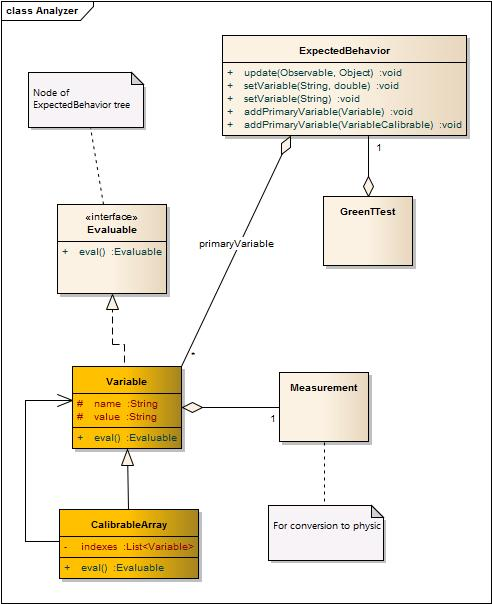
\includegraphics[width=9.8cm]{contents/images/eb.jpg}
\caption{Diagramme de classes d'une \textit{Expected Behavior}}
\label{fig:ebClasses}
\end{figure}
Figure \ref{fig:ebClasses} est disponible le diagramme de classes d'une \textit{Expected Behavior}, comme vous pouvez le voir, celle-ci possède un \texttt{evaluable} qui correspond à l'arbre d'expression logique. Elle a également une liste de variables primaires. L'arbre d'expression logique contient des références sur nos variables primaires, ainsi, si on effectue un \texttt{setValue} sur une variable donnée, alors cela modifiera correctement la valeur de la variable qui est dans l'\textit{Expected Behavior}.
\section{La maintenance}
Comme expliqué plus haut, j'ai développé deux fonctionnalités durant ce stage. Cependant, en parallèle de ce développement j'ai également corrigés différents bogues, ou améliorer différentes partie de la plateforme.

Ayant conçu cette plateforme lors de mon stage de fin de Licence, je connais l'intégralité de la plateforme. C'est ainsi que j'ai pu détecter et corriger un certains nombres de problèmes. Ceux-ci ont été identifiés de trois façons différentes : 
\begin{itemize}
	\item Durant mon développement, il m'est arrivé de trouver du code incohérent ou bouchonné
	\item Lors d'exécutions de la plateforme sur différentes versions du projet client
	\item En regardant les différents tickets\footnote{Nous avions une liste de <<tickets>> permettant de connaître les choses à faire sur le client, ou l'un des serveurs. Ces tickets peuvent être une action de maintenance, de \textit{refactoring}, une nouvelle fonctionnalité ou la correction d'un bug. Libre à chacun de mettre à jour ce document} ouverts et devant être résolus.
\end{itemize}

\subsection{Corrections}
J'ai corrigé quelques problèmes trouvés sur la plateforme, principalement venant du client \textit{GreenT}. Ceci étant dû à notre choix d'architecture : des serveurs les plus légers possibles et un client effectuant le maximum d'actions.
	\subsubsection{Stockage des erreurs d'exécutions}
	\begin{description}
		\item[Le problème] En cas d'erreur durant une exécution, si un serveur ne répond plus, si une variable est non trouvée, ... Une exception est levée. À ce moment là, \textit{GreenT} doit attraper l'exception et la stocker en base de données pour pouvoir afficher ensuite le message à tous les tests du bundle, la génération des rapports ne pouvant pas se faire.
		\item[La solution] Le stockage du message d'erreur n'était pas fait, ainsi que la requête SQL permettant d'obtenir les messages d'erreurs. Ces deux actions ont été corrigées, en lieu et place du rapport de test nous avons maintenant un message d'erreur clair lorsque le test n'a pas pu être exécuté.
		\end{description}
		
	\subsubsection{Modification des variables Debugger}
		\begin{description}
			\item[Le problème] Le serveur Trace32 doit pouvoir nous laisser modifier des variables présentes dans le logiciel du contrôle moteur. Or, lorsque nous appelions la commande de modification, celle-ci nous renvoyait systématiquement une exception.
			\item[La solution] Après lecture de la documentation de Trace32, il s'est avéré que le problème venait simplement du serveur qui appliquait une commande syntaxiquement incorrecte. La modification de la commande a corrigé le problème.
	\end{description}
	
	\subsubsection{Ordre d'exécutions des scénarios}
		\begin{description}
			\item[Le problème] Un Test peut contenir plusieurs scénarii, ceux-ci nous servent principalement pour le << patch-calib >> comme expliqué section \ref{patch}. Or, si nous utilisions plusieurs scénarii, ceux-ci étaient exécutés dans un ordre aléatoire : il n'était pas possible de les exécuter dans un ordre donné.
			\item[La solution] Le problème avait deux parties : d'une part, l'exécution des scénarii dans un ordre donné, d'autre part, spécifier un ordre à chacun de nos scénarii. En effet, tout d'abord, j'ai nommé les scénarii de sortes qu'ils soient classés par ordre alphabétique. Ensuite, il a fallu spécifier à la plateforme d'exécuter ceux-ci dans un ordre alphabétique, pour cela il a suffit d'utiliser une collection Java effectuant cette action, la \texttt{TreeMap}.
	\end{description}
	
	\subsubsection{Reset ECU à l'exécution}
	\begin{description}
		\item[Le problème] Lors de l'exécution de notre plateforme sur la dernière version du projet client, nous avions systématiquement un \textit{reset} ECU. C'est-à-dire que notre ECU s'arrêtait et ne redémarrait pas pour une raison inconnue.
		\item[La solution] Le problème ne venait pas directement de la plateforme, mais d'une mauvaise configuration de notre part. En effet, nous ne spécifiions pas les bons fichiers du logiciel, celui-ci étant mal flashé, l'ECU refusait de démarrer.
	\end{description}
	
	\subsubsection{Absence d'injection}
	\begin{description}
		\item[Le problème] Lorsque j'essayais de simuler un démarrage du moteur sur la dernière version du logiciel, aucune injection ne se faisait : après le starter, le moteur retournait à zéro tour par minute.
		\item[La solution] Après s'être renseigné auprès de personnes compétentes, il s'est avéré que cela venait d'un nouveau fichier à flasher dont nous n'avions pas connaissance. Un fichier contenant des calibrations permettant le démarrage du moteur sur table. Ce fichier n'ayant pas été pris en compte durant la conception, j'ai ajouté un nouveau paramètre au fichier de configuration permettant de renseigner des fichiers à flasher additionnels.
	\end{description}
	
\subsection{Améliorations}
	\subsubsection{Exécution différée} %
	\begin{description}
		\item[Le besoin] Lors de mon développement, j'ai eu souvent des problèmes pour réserver des tables de tests. Celles-ci étant régulièrement prise par les équipes projets. 
		\item[La solution] Afin de ne pas bloquer de tables, et de ne pas retarder notre travail en raison de l'absence de celles-ci, une solution nous est venue : la possibilité de lancer l'outil durant la nuit. En effet, actuellement une exécution dure environ 45 minutes pour 80 tests, après laquelle nous pouvons analyser les rapports et voir les problèmes qui nous sont retournés. Ainsi, j'ai ajouté un nouveau paramètre à l'application permettant de spécifier l'heure à laquelle la génération des \texttt{.jar}, la compilation, l'exécution et la génération des rapports va se faire. On peut maintenant lancer une exécution le soir et observer les résultats le lendemain matin.
	\end{description}
	
	\subsubsection{Passage à Java 8}
		\begin{description}
			\item[Le besoin] La plateforme fonctionnait sous Java 6. Ainsi, nous allions mettre en production une plateforme déjà obsolète à sa sortie. De plus, les deux versions suivantes de Java proposent un certain nombre de fonctionnalités aidant au développement, comme des simplifications d'écriture en Java 7 (\textit{Multi-Catch}, Inférence de type, \texttt{switch} sur les strings, ...) ou les lambdas-calculs en Java 8. Enfin, dans un futur proche nous aurons besoin d'une interface pour \textit{GreenT}, \texttt{JavaFx} serait une bonne solution, mais celle-ci nécessite Java 8.
			\item[La solution] Avant de passer à Java 8, il a d'abord fallut vérifier qu'aucune incompatibilité avec les bibliothèques que nous utilisons n'allait apparaître. Ensuite, il était nécessaire de télécharger un compilateur ainsi qu'une JVM, configurer les différents environnements et vérifier qu'une exécution se passait de la même manière que précédemment. Après ce succès, le passage à Java 8 a été concrétisé et permet à notre plateforme de rester moderne ! 
		\end{description}
		
	\subsubsection{<< \textit{Clean-Code} >>}
		\begin{description}
			\item[Le besoin] \textit{GreenT} ayant deux ans, et ayant connue quatre développeurs différents, il est parfois nécessaire d'améliorer le code existant ou de le rendre plus lisible. 
			\item[La solution] Lorsqu'en développant mes fonctionnalités ou en corrigeant des bogues je rencontrais du code incompréhensible ou du << code mort >>, je modifiais celui-ci afin de corriger ces défauts. Ceci permet ainsi de garder un code toujours propre et facile à lire.
		\end{description}
		
	\subsubsection{Affichage des \textit{logs}}
		\begin{description}
			\item[Le besoin] La plateforme effectue beaucoup d'actions, allant du parsing jusqu'à la génération des rapports comme montré chapitre \ref{chapGreent}. Toutes ces actions doivent être tracées, aussi bien en temps réel, en regardant l'exécution, que plus tard en observant un fichier.
			\item[La solution] Les logs fonctionnait déjà, en utilisant \texttt{log4j}, cependant celui-ci affichait beaucoup trop d'informations en temps réel, et n'affichait pas les informations les plus utiles. Ainsi, j'ai passé en revue la plateforme pour afficher les bonnes actions (Initialisation des bancs, stimulis effectués, affichage des exceptions, \ldots). Toutes les erreurs sont redirigées vers la sortie des erreurs (\texttt{stderr}), et seules les informations les plus importantes sont sur la sortie console (\texttt{stdout}). Tous les autres logs, qui peuvent être utile à la compréhension d'un problème et nous aider ne sont accessible que dans nos fichiers de logs. J'ai par ailleurs ajouté un « buffer tournant » permettant aux fichiers de logs de ne jamais dépasser une certaines taille (5Mio), afin de ne pas consommer trop d'espace disque.
		\end{description}
		

